The GAs were applied to the selection of features for the prediction
of effective temperature from both, noiseless and noisy spectra.  For
the IRTF wavelength range and resolution, results in the features have
been included in Table~\ref{tab:irtf-teff-noisy}. Features are ordered
by the fitness value (according to the AIC criterion, as explained in
Eq.~\ref{eq:AIC}) and we only consider features that are present in at
least 5 sets.

Table \ref{tab:irtf-teff-noisy} shows a very wide variety of features
with very few repetitions. Only spectral features 4, 5, 6, and 9 in
the SNR=50 experiment are found too in the SNR=$\infty$ and SNR=10
feature sets (albeit with different continuum definitions). This
reinforces the impression that the information useful for the
estimation of the effective temperatures is spread over the entire
IRTF spectrum.

\begin{figure*}
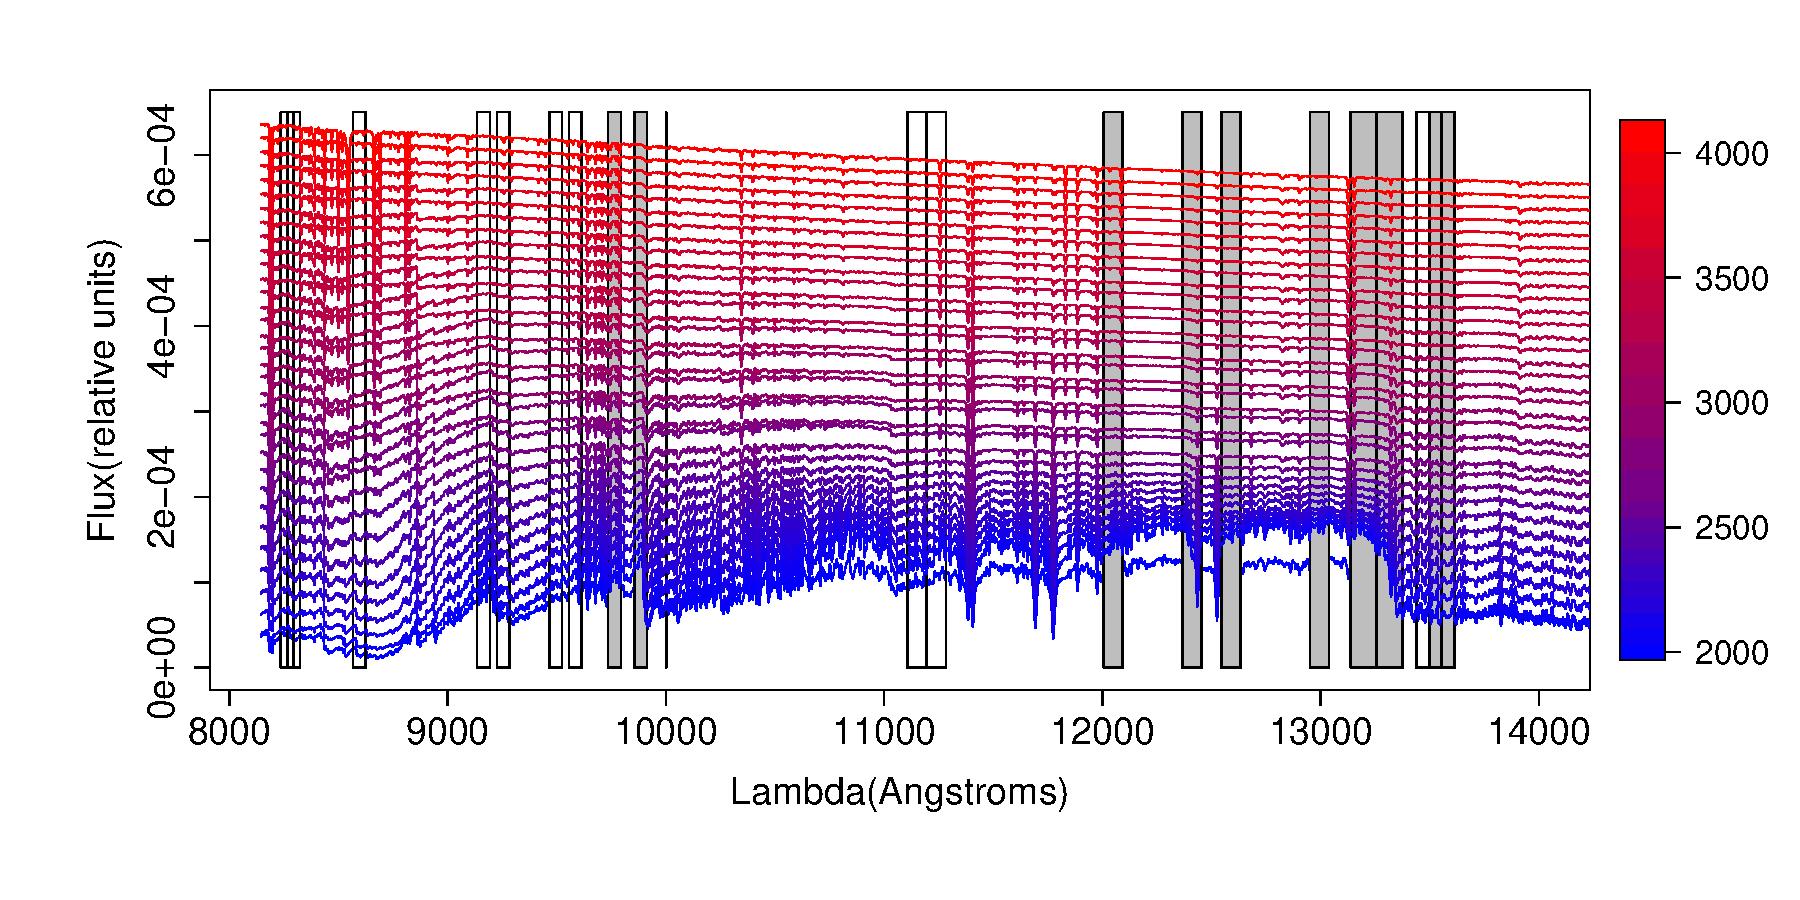
\includegraphics[width=\textwidth]{figs/BT-spectraAtIRTF-Inf-teff2}
 \caption{Features selected by the GA for predicting $T_{eff}$ using
    noiseless BT\_Settl synthetic spectra in the IRTF wavelength range
    and resolution. The BT\ Settl spectra are plot in a colour scale
    that ranges from blue (2000 K) to red (4100 K). The empty boxes
    correspond to the selected features and the grey boxes to the
    continuum bands.}  \label{fig:IRTF-teff}
\end{figure*}

For gravity estimation (on a logarithmic scale) and metallicity,
the GA search procedure produces the features presented in Tables
\ref{tab:irtf-logg-noisy} and \ref{tab:irtf-met-noisy}
respectively. Figure \ref{fig:IRTF-teff} shows a graphical
representation of the bands selected for the determination of the
effective temperature superimposed on a set of noiseless BT Settl
spectra.

